\chapter{Transitions de phase}\label{ch:b3:phase-transitions}

Chauffez de l'eau d'un degré et il ne se passe pas grand-chose ---
jusqu'à ce que, à une température nettement définie, le liquide se
déchire en vapeur. Refroidissez du fer à travers \qty{1043}{K} et,
sans changement de composition, il s'aimante spontanément. Rien dans
une molécule seule ni dans un spin seul n'annonce ces révolutions~:
elles sont \emph{collectives} --- $10^{23}$ agents, chacun en
interaction avec quelques voisins, conspirant à changer d'un coup la
phase de leur société. Le volume de première année a catalogué les
transitions~; ce chapitre en explique le mécanisme avec les outils
des cinq derniers~: compétition d'\omterm{prop:b3:canonical-ensemble:machine}{énergie libre}, \omterm{def:b3:phase-transitions:order}{paramètres d'ordre},
\omterm{def:b3:phase-transitions:order}{brisure de symétrie}, et la stupéfiante découverte qu'au voisinage
d'un \omterm{prop:b3:phase-transitions:vdw}{point critique} les détails microscopiques cessent de compter
--- un aimant et un fluide bouillant partagent les mêmes \omterm{prop:b3:phase-transitions:landau}{exposants
critiques}. Les idées de ce chapitre courent aujourd'hui des
autocuiseurs aux supraconducteurs jusqu'au champ de Higgs du
\cref{ch:b3:particle-physics}.

\section{Paramètres d'ordre et compétition d'énergie libre}

\begin{definition}[Phases et paramètres d'ordre]\label{def:b3:phase-transitions:order}
\index{transition de phase}\index{paramètre d'ordre}\index{brisure de symétrie}
Une \emph{transition de phase} est un changement non régulier de
l'état d'équilibre d'un système lorsqu'un paramètre de contrôle
($T$, $P$, $B$) franchit une frontière. Son comptable est le
\emph{paramètre d'ordre}~: une grandeur nulle dans la phase
désordonnée et non nulle dans la phase ordonnée --- l'aimantation
$m$ d'un ferroaimant, la différence de densité
$\rho_{\text{liq}} - \rho_{\text{gaz}}$ d'un fluide, la fraction
condensée du \cref{ch:b3:quantum-statistics}. Les transitions sont
de deux sortes~: du \emph{premier ordre} (le paramètre d'ordre
saute~; chaleur latente~; les phases coexistent --- ébullition,
fusion) et \emph{continues} (le paramètre d'ordre croît depuis
zéro~; pas de chaleur latente~; fluctuations déchaînées --- le point
de Curie, le \omterm{prop:b3:phase-transitions:vdw}{point critique}, l'hélium superfluide). Quand l'état
ordonné doit \emph{choisir} parmi des options équivalentes --- le
nord d'un aimant doit bien pointer quelque part --- la transition
\emph{brise une symétrie} que les lois sous-jacentes respectent~:
thème qui reviendra, aux enjeux les plus hauts, avec le mécanisme de
Higgs. Le moteur derrière chaque cas est l'\omterm{prop:b3:canonical-ensemble:machine}{énergie libre} $F = E - TS$
(\cref{prop:b3:canonical-ensemble:machine})~: l'énergie favorise
l'ordre, l'entropie favorise le désordre, et $T$ fixe le taux de
change --- les frontières de phase sont là où les comptes s'égalisent.
\end{definition}

\section{La transition liquide--gaz~: van der Waals}

\begin{proposition}[Isothermes de van der Waals]\label{prop:b3:phase-transitions:vdw}
\index{équation de van der Waals}\index{point critique}
L'équation des gaz réels du volume de première année,
\[
\Big(P + \frac{aN^2}{V^2}\Big)(V - Nb) = Nk_{\text{B}}T ,
\]
encode l'attraction ($a$) et les cœurs durs ($b$). Au-dessus d'une
température critique $T_{\text{c}} = 8a/27bk_{\text{B}}$ ses
isothermes sont monotones~: une seule phase fluide. Au-dessous,
elles développent une boucle contenant une portion mécaniquement
\emph{instable} ($\partial P/\partial V >
0$)~: le fluide s'y sépare en liquide et gaz coexistants, à la
pression fixée par l'égalité des \omterm{thm:b3:grand-canonical:distribution}{potentiels chimiques} (règle des
aires égales de Maxwell). Le domaine de coexistence se referme au
\omterm{prop:b3:phase-transitions:vdw}{point critique} ($P_{\text{c}}, V_{\text{c}}, T_{\text{c}}$), où
liquide et gaz deviennent \emph{indiscernables}~: en s'en
approchant, la différence de densité s'annule, la compressibilité
diverge, et les fluctuations de densité atteignent la taille
optique --- l'opalescence critique de
\cref{pb:b3:perturbation-theory:1}.
\end{proposition}
\admitted

\begin{omfigure}
\begin{tikzpicture}
  \begin{axis}[omaxis, axis x line=bottom, axis y line=left,
    width=10.8cm, height=6.0cm, xmin=0.32, xmax=5, ymin=0, ymax=2.1,
    xlabel={$V/V_{\text{c}}$}, ylabel={$P/P_{\text{c}}$},
    xlabel style={at={(axis description cs:0.5,-0.09)}, anchor=north},
    xtick={1,2,3,4}, ytick={1}, clip=true,
    legend pos=north east,
    legend style={font=\scriptsize, draw=none, fill=none}]
    % reduced vdw: P = 8T/(3V-1) - 3/V^2 (T in units of Tc)
    \addplot[omDef, very thick, domain=0.42:5, samples=250]
      {8*1.05/(3*x-1) - 3/(x*x)};
    \addplot[omThm, very thick, domain=0.42:5, samples=250]
      {8/(3*x-1) - 3/(x*x)};
    \addplot[omExo, very thick, domain=0.44:5, samples=300]
      {8*0.9/(3*x-1) - 3/(x*x)};
    \legend{$T > T_{\text{c}}$, $T = T_{\text{c}}$, $T < T_{\text{c}}$}
    % coexistence dome (schematic)
    \addplot[gray, dashed, domain=0.5:2.9, samples=100, forget plot]
      {1 - 0.62*(ln(x/1.06))^2};
    \fill (axis cs:1,1) circle (1.8pt);
    \draw[gray, ->] (axis cs:1.55,1.5) -- (axis cs:1.05,1.06);
    \node[font=\scriptsize, anchor=west] at (axis cs:1.6,1.55)
      {point critique};
    \node[gray, font=\scriptsize, anchor=north] at (axis cs:1.7,0.62)
      {dôme de coexistence};
  \end{axis}
\end{tikzpicture}

{\small Isothermes de van der Waals en unités réduites. Au-dessus de
$T_{\text{c}}$~: un seul fluide. Au-dessous~: le milieu instable de
la boucle est remplacé par la coexistence diphasique plate à
l'intérieur du dôme en tirets. Au sommet du dôme, liquide et gaz
fusionnent --- le \omterm{prop:b3:phase-transitions:vdw}{point critique}, où les fluctuations rendent le
fluide laiteux.}
\end{omfigure}

\begin{proposition}[Clausius--Clapeyron]\label{prop:b3:phase-transitions:clapeyron}
\index{relation de Clausius--Clapeyron}
Le long de toute ligne de coexistence du premier ordre, l'égalité
des \omterm{thm:b3:grand-canonical:distribution}{potentiels chimiques} de part et d'autre
(\cref{def:b3:grand-canonical:mu}) impose à la pente de la ligne
\[
\frac{\dd P}{\dd T} = \frac{L}{T\,\Delta v} ,
\]
avec $L$ la chaleur latente et $\Delta v$ le changement de volume par
particule (ou par kilogramme, de façon cohérente). Tout ce qui
concerne les lignes de coexistence tient dans cette seule formule~:
la ligne d'ébullition de l'eau monte de
$\approx\qty{3.6}{kPa/K}$ près de \qty{100}{\celsius}
(autocuiseurs, cuisine en altitude ---
\cref{pb:b3:phase-transitions:1})~; et la ligne de \emph{fusion} de
l'eau penche à l'envers ($\Delta v < 0$~: la glace flotte), si bien
que la pression fait fondre la glace --- une rareté parmi les
substances, aux conséquences allant des glaciers aux patinoires.
\end{proposition}

\begin{proof}
Sur la ligne, $\mu_1(T, P) = \mu_2(T, P)$~; déplaçons-nous le long~:
$-s_1\dd T + v_1\dd P = -s_2\dd T + v_2\dd P$ (par particule, avec
$\dd\mu = -s\,\dd T + v\,\dd P$). Résolvons en $\dd P/\dd T$ et
utilisons $L = T(s_2 - s_1)$.
\end{proof}

\section{Le ferroaimant~: la théorie de champ moyen}

\begin{theorem}[Transition d'Ising en champ moyen]\label{thm:b3:phase-transitions:meanfield}
\index{modèle d'Ising}\index{théorie de champ moyen}\index{température de Curie}
Modélisez un aimant par des spins $s_i = \pm1$ sur un réseau, les
voisins couplés par l'énergie d'échange $-J\,s_is_j$
(\cref{exo:b3:identical-particles:12}), chaque spin ayant $q$
voisins. Remplacez les voisins de chaque spin par leur moyenne $m =
\langle s\rangle$ (l'approximation de \emph{champ moyen})~: un spin
siège alors dans le champ effectif $qJm$, et
\cref{exo:b3:canonical-ensemble:11} donne la condition
d'auto-cohérence
\[
m = \tanh\!\Big(\frac{T_{\text{c}}}{T}\,m\Big) , \qquad
k_{\text{B}}T_{\text{c}} = qJ .
\]
Au-dessus de $T_{\text{c}}$ la seule solution est $m = 0$~;
au-dessous, deux solutions symétriques $\pm m(T)$ apparaissent et
sont les solutions stables~: l'aimant \emph{doit} s'aimanter, en
choisissant une direction au hasard --- brisure spontanée de
symétrie. Près de $T_{\text{c}}$, $m \propto
(T_{\text{c}} - T)^{1/2}$, et au-dessus la susceptibilité obéit à
la loi de Curie--Weiss $\chi \propto 1/(T - T_{\text{c}})$~:
divergente à la transition --- un aimant infiniment complaisant.
\end{theorem}

\begin{proof}[Démonstration partielle]
Un spin dans le champ $B_{\text{eff}} = qJm/\mu$ a $\langle s\rangle =
\tanh(\beta qJm)$~; exiger $\langle s\rangle = m$ donne l'équation
annoncée. Graphiquement~: la droite $y = m$ coupe la courbe $y =
\tanh(T_{\text{c}}m/T)$ seulement à l'origine quand la pente
initiale de la courbe vérifie $T_{\text{c}}/T < 1$, et aussi en
$\pm m^* \neq 0$ quand $T < T_{\text{c}}$. Développer $\tanh$ pour
$m$ petit donne $m^2 = 3(1 - T/T_{\text{c}})$, la croissance en
racine carrée~; ajouter un petit champ appliqué et développer de
même donne Curie--Weiss (\cref{exo:b3:phase-transitions:6}).
\end{proof}

\begin{omfigure}
\begin{tikzpicture}
  \begin{axis}[omaxis, axis x line=bottom, axis y line=left,
    width=6.6cm, height=5.2cm, xmin=0, xmax=1.6, ymin=0, ymax=1.15,
    xlabel={$m$}, ylabel={},
    xlabel style={at={(axis description cs:0.5,-0.11)}, anchor=north},
    xtick=\empty, ytick=\empty, clip=false]
    \addplot[gray, thick, domain=0:1.1] {x};
    \addplot[omDef, very thick, domain=0:1.6, samples=100]
      {tanh(1.5*x)};
    \addplot[omExo, thick, dashed, domain=0:1.6, samples=100]
      {tanh(0.7*x)};
    \fill[omDef] (axis cs:0.858,0.858) circle (1.8pt);
    \node[omDef, font=\scriptsize, anchor=north west] at (axis cs:0.88,0.84)
      {$m^*$};
    \node[omDef, font=\scriptsize, anchor=south east] at (axis cs:1.55,1.0)
      {$T < T_{\text{c}}$};
    \node[omExo, font=\scriptsize, anchor=north] at (axis cs:1.32,0.62)
      {$T > T_{\text{c}}$};
    \node[gray, font=\scriptsize, anchor=west, rotate=38] at (axis cs:0.3,0.38)
      {$y = m$};
  \end{axis}
  \begin{axis}[omaxis, axis x line=bottom, axis y line=left,
    width=6.6cm, height=5.2cm, xmin=0, xmax=1.25, ymin=0, ymax=1.15,
    xshift=7.2cm,
    xlabel={$T/T_{\text{c}}$}, ylabel={$m(T)$},
    xlabel style={at={(axis description cs:0.5,-0.11)}, anchor=north},
    xtick={0.5,1}, ytick={1}, clip=false]
    \addplot[omThm, very thick, domain=0.02:0.999, samples=250]
      {(1-x^3.4)^0.42};
    \addplot[omThm, very thick, domain=1:1.18] {0};
    \node[omThm, font=\scriptsize, anchor=east] at (axis cs:0.88,0.45)
      {$\propto(T_{\text{c}} - T)^{1/2}$ near $T_{\text{c}}$};
  \end{axis}
\end{tikzpicture}

{\small À gauche~: l'auto-cohérence $m = \tanh(T_{\text{c}}m/T)$ ---
au-dessous de $T_{\text{c}}$ la pente initiale de la courbe dépasse
un et un croisement non nul $m^*$ existe. À droite~: l'aimantation
spontanée qui en résulte, croissant en racine carrée sous le point
de Curie et identiquement nulle au-dessus.}
\end{omfigure}

\section{Le point de vue de Landau et l'universalité}

\begin{proposition}[Théorie de Landau]\label{prop:b3:phase-transitions:landau}
\index{théorie de Landau}\index{exposants critiques}\index{universalité}
Près d'une transition continue, développer l'\omterm{prop:b3:canonical-ensemble:machine}{énergie libre} en le
petit \omterm{def:b3:phase-transitions:order}{paramètre d'ordre}, en ne gardant que ce que la symétrie
autorise ($m \to -m$ ici)~:
\[
F(m) = a\,(T - T_{\text{c}})\,m^2 + b\,m^4 , \qquad a, b > 0 .
\]
Au-dessus de $T_{\text{c}}$~: un seul puits en $m = 0$. Au-dessous~:
l'origine devient un sommet et deux puits symétriques apparaissent
en $m = \pm
\sqrt{a(T_{\text{c}} - T)/2b}$ --- la même racine carrée qu'en champ
moyen, issue maintenant de la seule symétrie. Voilà pourquoi des
systèmes très différents se comportent identiquement près de leurs
\omterm{prop:b3:phase-transitions:vdw}{points critiques}~: l'\emph{universalité}. Les exposants mesurés (par
exemple $m \propto |T -
T_{\text{c}}|^\beta$ avec $\beta \approx 0.33$ à la fois pour les
fluides \emph{et} pour les aimants uniaxiaux) diffèrent du $1/2$ de
champ moyen parce que, près de $T_{\text{c}}$, les fluctuations font
rage à toutes les échelles --- leur domestication, le groupe de
renormalisation (Wilson, Nobel 1982), a montré que seules la
dimensionnalité et la symétrie, jamais les détails microscopiques,
décident des exposants. L'image du double puits a elle-même une
carrière au-delà des aimants~: donner au \omterm{def:b3:phase-transitions:order}{paramètre d'ordre} le rôle
d'un champ emplissant l'espace, et son puits à symétrie brisée est
le mécanisme de Higgs (\cref{ch:b3:particle-physics}).
\end{proposition}
\admitted

\begin{omfigure}
\begin{tikzpicture}
  \begin{axis}[omaxis, axis x line=bottom, axis y line=left,
    width=11.6cm, height=5.2cm, xmin=-1.6, xmax=1.6, ymin=-0.45, ymax=0.85,
    xlabel={paramètre d'ordre $m$}, ylabel={$F(m)$},
    xlabel style={at={(axis description cs:0.5,-0.11)}, anchor=north},
    xtick={0}, ytick=\empty, clip=false,
    legend style={font=\scriptsize, at={(0.5,0.98)}, anchor=north,
      draw=none, fill=none}]
    \addplot[omDef, very thick, domain=-1.07:1.07, samples=120]
      {0.5*x*x + 0.2*x^4};
    \addlegendentry{$T > T_{\text{c}}$~: un puits}
    \addplot[omExo, thick, domain=-1.31:1.31, samples=120]
      {0.28*x^4};
    \addlegendentry{$T = T_{\text{c}}$~: fond plat}
    \addplot[omThm, very thick, domain=-1.6:1.6, samples=150]
      {-0.55*x*x + 0.28*x^4 + 0.27};
    \addlegendentry{$T < T_{\text{c}}$~: deux puits}
    \fill[omThm] (axis cs:0.99,0.0) circle (1.6pt);
    \fill[omThm] (axis cs:-0.99,0.0) circle (1.6pt);
  \end{axis}
\end{tikzpicture}

{\small L'\omterm{prop:b3:canonical-ensemble:machine}{énergie libre} de Landau~: refroidir à travers
$T_{\text{c}}$ change un puits en deux. Le système doit rouler dans
l'un d'eux --- équivalents par symétrie, distincts en fait~:
brisure spontanée de symétrie, des aimants au champ de Higgs.}
\end{omfigure}

\begin{method}[Lire une transition]\label{met:b3:phase-transitions:method}
(1) Identifier le \omterm{def:b3:phase-transitions:order}{paramètre d'ordre} et s'il saute (premier ordre~:
chaleur latente, coexistence, hystérésis, nucléation) ou s'il croît
continûment (\omterm{prop:b3:phase-transitions:vdw}{point critique}~: divergences, opalescence,
universalité). (2) Lignes du premier ordre~: Clausius--Clapeyron
pour la pente~; l'égalité des $\mu$ pour la coexistence. (3)
Continues~: le champ moyen d'abord ($\tanh$ ou Landau) pour la forme
du diagramme de phases~; se fier à sa \emph{topologie}, non à ses
exposants. (4) Sous $T_{\text{c}}$, se rappeler le choix~: symétrie
brisée signifie domaines, défauts et dépendance à l'histoire. (5)
Estimations~: $k_{\text{B}}T_{\text{c}} \sim$ (couplage par voisin)
$\times$ (nombre de voisins).
\end{method}

\begin{omfigure}
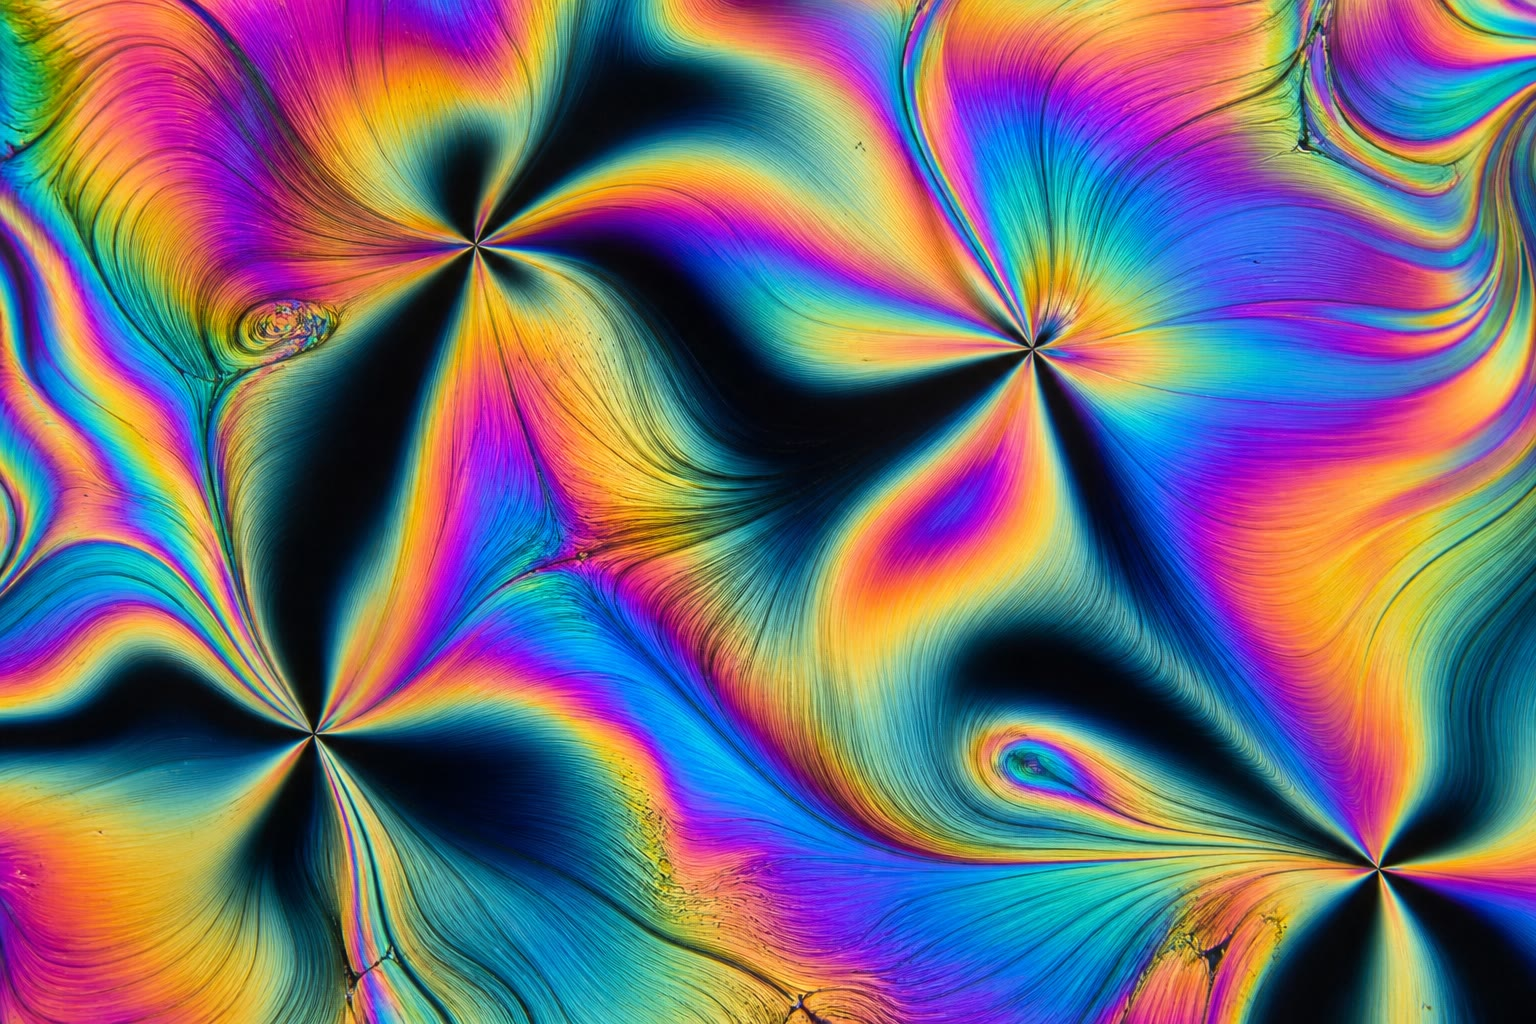
\includegraphics[width=0.58\linewidth]{images/book5/ai/b5-26-liquid-crystal.jpg}

{\small Un cristal liquide entre polariseurs croisés~: un \omterm{def:b3:phase-transitions:order}{paramètre d'ordre} (l'axe moléculaire) tourbillonnant à travers les défauts où les brosses se rejoignent. Les phases de la matière entre liquide et solide --- et la substance active de la plupart des écrans.}
\end{omfigure}

\section{Exercices}

\begin{exercise}[$\star$]\label{exo:b3:phase-transitions:1}
Classer (premier ordre ou continue), en nommant le \omterm{def:b3:phase-transitions:order}{paramètre d'ordre}
et la symétrie brisée s'il y en a une~: (a) l'ébullition à
\qty{1}{atm}~; (b) le point de Curie~; (c) le point $\lambda$
superfluide~; (d) l'ébullition \emph{exactement au} \omterm{prop:b3:phase-transitions:vdw}{point critique}.
\end{exercise}

\begin{exercise}[$\star$]\label{exo:b3:phase-transitions:2}
Les chaleurs latentes vues comme entropie. (a) L'eau~: $L_{\text{vap}} =
\qty{2.26e6}{J/kg}$ à \qty{373}{K}~: calculer le $\Delta S$ par
molécule en unités de $k_{\text{B}}$. (b) Idem pour la fusion
($L_{\text{fus}} = \qty{3.3e5}{J/kg}$ à \qty{273}{K}). (c) La
plupart des liquides se vaporisent avec
$\Delta S \approx 10$--$11\,k_{\text{B}}$ (règle de Trouton)~: que
compte approximativement ce nombre (le $\ln$ de quel rapport de
volumes)~? (d) Pourquoi le saut d'entropie de la fusion est-il si
inférieur à celui de l'ébullition~?
\end{exercise}

\begin{exercise}[$\star$]\label{exo:b3:phase-transitions:3}
Constantes critiques de van der Waals ($V_{\text{c}} = 3Nb$,
$k_{\text{B}}T_{\text{c}} = 8a/27b$, $P_{\text{c}} = a/27b^2$ ---
admises). (a) Montrer que $P_{\text{c}}V_{\text{c}}/Nk_{\text{B}}T_{\text{
c}} = 3/8$, un nombre universel pour le modèle~; les valeurs
mesurées se groupent près de $0.29$ --- commenter. (b) Pour le
CO$_2$ ($T_{\text{c}} = \qty{304}{K}$,
$P_{\text{c}} = \qty{73.8}{bar}$)~: extraire $a$ et $b$. (c) À
partir de $b$, estimer le diamètre moléculaire. (d) Pourquoi le
CO$_2$ à température ambiante se liquéfie-t-il sous pression tandis
que le N$_2$ à température ambiante ($T_{\text{c}} =
\qty{126}{K}$) ne le fait jamais~?
\end{exercise}

\begin{exercise}[$\star$]\label{exo:b3:phase-transitions:4}
Des \omterm{def:b3:phase-transitions:order}{paramètres d'ordre}, rapidement~: en donner un pour (a) un
ferroaimant~; (b) la transition liquide--gaz~; (c) la \omterm{thm:b3:quantum-statistics:bec}{condensation
de Bose--Einstein}~; (d) un antiferroaimant (deux sous-réseaux ---
quelle grandeur s'ordonne alors que l'aimantation totale reste
nulle~?).
\end{exercise}

\begin{exercise}[$\star\star$]\label{exo:b3:phase-transitions:5}
Le champ moyen à la main. (a) Obtenir $m = \tanh(\beta qJm)$ pour
un spin dans le champ moyen de ses $q$ voisins. (b) Montrer qu'une
solution non nulle existe exactement quand $T < qJ/k_{\text{B}}$.
(c) Développer au troisième ordre et obtenir $m(T) \approx \sqrt{3(1 -
T/T_{\text{c}})}$. (d) Le fer~: $T_{\text{c}} = \qty{1043}{K}$, $q =
8$~: extraire $J$ en eV et vérifier l'échelle d'échange de
\cref{exo:b3:identical-particles:12}.
\end{exercise}

\begin{exercise}[$\star\star$]\label{exo:b3:phase-transitions:6}
Curie--Weiss. Ajouter un petit champ~: $m = \tanh[\beta(qJm + \mu B)]$.
(a) Linéariser au-dessus de $T_{\text{c}}$ et obtenir $\chi = \partial
m/\partial B \propto 1/(T - T_{\text{c}})$. (b) Comparer à la loi de
Curie des spins libres~: que donne le tracé de $1/\chi$ contre $T$
dans chaque cas, et comment l'ordonnée à l'origine diagnostique-t-elle
un couplage ferromagnétique~? (c) La droite $1/\chi$ du nickel touche
zéro à \qty{631}{K}~: interpréter. (d) Pour un antiferroaimant,
l'ordonnée à l'origine est \emph{négative}~: quel signe de $J$ cela
trahit-il~?
\end{exercise}

\begin{exercise}[$\star\star$]\label{exo:b3:phase-transitions:7}
Clausius--Clapeyron à l'œuvre. (a) L'eau à \qty{100}{\celsius}
($\Delta v = \qty{1.67}{m^3/kg}$)~: calculer $\dd P/\dd T$. (b)
Utiliser $\dd\ln P/\dd T = Lm_{\text{w}}/k_{\text{B}}T^2$ pour
estimer la température d'ébullition à $P = \qty{0.7}{atm}$ (un
sommet à \qty{3000}{m}). (c) Fusion~: avec
$\Delta v = \qty{-9.1e-5}{m^3/kg}$ et $L = \qty{3.3e5}{J/kg}$,
calculer $\dd T/\dd P$ et la pression qui abaisse le point de fusion
de la glace de \qty{5}{K}. (d) Un patineur de \qty{70}{kg} sur
\qty{30}{mm^2} de lame~: la pression et le décalage du point de
fusion --- la fusion sous pression explique-t-elle le patinage~? (Ce
qui l'explique~: le frottement et la préfusion de surface.)
\end{exercise}

\begin{exercise}[$\star\star$]\label{exo:b3:phase-transitions:8}
Calculs de Landau. (a) Minimiser $F = a(T - T_{\text{c}})m^2 +
bm^4$ au-dessous de $T_{\text{c}}$. (b) Calculer $F$ au minimum et
montrer que la capacité thermique présente un \emph{saut} fini $\Delta C =
a^2T_{\text{c}}/2b$ à la transition. (c) Esquisser $C(T)$~: la
marche de champ moyen contre le pic quasi logarithmique mesuré au
point $\lambda$ de l'hélium --- qu'ajoutent les vraies
fluctuations~? (d) Ajouter un terme de champ $-hm$~: montrer que la
transition s'arrondit --- la symétrie doit être exacte pour être
brisée.
\end{exercise}

\begin{exercise}[$\star\star$]\label{exo:b3:phase-transitions:9}
Nucléation. Une gouttelette de rayon $r$ dans une vapeur sursaturée
gagne l'\omterm{prop:b3:canonical-ensemble:machine}{énergie libre} de volume $-\tfrac43\pi r^3\,n\,\delta\mu$
mais paie la tension superficielle $4\pi r^2\sigma$. (a) Montrer que
la barrière culmine en $r^* = 2\sigma/n\,\delta\mu$. (b)
Expliquer~: pourquoi les vapeurs sursaturées propres et les liquides
surchauffés persistent-ils (métastabilité), et qu'apportent les
poussières, les ions et les rayures~? (c) Les chambres à brouillard
(les détecteurs ancêtres du \cref{ch:b3:particle-physics}) et les
chambres à bulles fonctionnent \emph{sur} cette physique~: quel rôle
joue la traînée d'ions de la particule qui passe~? (d) Pourquoi
met-on des «~régulateurs d'ébullition~» dans les ballons de
laboratoire~?
\end{exercise}

\begin{exercise}[$\star\star\star$]\label{exo:b3:phase-transitions:10}
Pas de transition à une dimension. Considérer une chaîne d'Ising 1D
de $N$ spins, tous en haut, et insérer une «~paroi de domaine~»
(tous les spins au-delà d'une liaison retournés). (a) Coût en
énergie de la paroi~: $2J$, indépendant de la position. (b) Gain
d'entropie~: la paroi peut siéger sur l'une des $\sim N$ liaisons
--- $\Delta S = k_{\text{B}}\ln N$. (c) Montrer que
$\Delta F = 2J - k_{\text{B}}T\ln N < 0$ pour tout $T > 0$ à grand
$N$~: les parois prolifèrent toujours, et l'ordre à longue portée
est impossible --- le \omterm{thm:b3:phase-transitions:meanfield}{modèle d'Ising} 1D a $T_{\text{c}} = 0$. (d) À
2D, une paroi est une ligne de longueur $\ell$ coûtant $2J\ell$ mais
avec $\sim3^\ell$ formes~: refaites l'estimation et montrer que
l'ordre \emph{survit} au-dessous d'un $T_{\text{c}}$ fini ---
l'argument de Peierls derrière le $2.269\,J/k_{\text{B}}$ exact
d'Onsager.
\end{exercise}

\begin{exercise}[$\star\star\star$]\label{exo:b3:phase-transitions:11}
L'universalité auditée. Le champ moyen prédit $\beta = 1/2$, $\gamma
= 1$ ($\chi \sim |t|^{-\gamma}$), $\delta = 3$ ($m \sim h^{1/3}$
en $T_{\text{c}}$). Mesuré, pour le \omterm{prop:b3:phase-transitions:vdw}{point critique} liquide--gaz
\emph{comme} pour les aimants uniaxiaux tridimensionnels~: $\beta
\approx 0.326$, $\gamma \approx 1.237$, $\delta \approx 4.79$.
(a) Qu'est-ce qui autorise à comparer un fluide et un aimant (que
partagent leurs \omterm{def:b3:phase-transitions:order}{paramètres d'ordre} --- un unique choix de signe)~?
(b) Pourquoi le champ moyen échoue-t-il près de $T_{\text{c}}$
(qu'est-ce qui diverge, invalidant l'abandon des fluctuations)~? (c)
Pourquoi échoue-t-il \emph{moins} en dimension plus élevée (nombre
de voisins contre portée des fluctuations~; le champ moyen devient
exact au-dessus de quatre dimensions)~? (d) Énoncer en deux phrases
la morale du groupe de renormalisation~: sur quoi moyenne-t-on
échelle par échelle, et pourquoi seules la symétrie et la dimension
survivent à cette moyenne.
\end{exercise}

\begin{exercise}[$\star\star\star$]\label{exo:b3:phase-transitions:12}
Des aimants au Higgs. Promouvoir le \omterm{def:b3:phase-transitions:order}{paramètre d'ordre} au rang de
champ $\phi(\vect r)$ de densité d'énergie de Landau $\alpha(T -
T_{\text{c}})\phi^2 + b\phi^4$ plus un terme de gradient. (a)
Au-dessous de $T_{\text{c}}$ le champ siège en $\pm\phi_0$~: les
\omterm{prop:b3:lagrangian-mechanics:modes}{petites oscillations} \emph{le long} du puits ont une courbure de
rappel --- calculer $F''(\phi_0)$ et l'interpréter, en langage de
champs, comme une \emph{masse}. (b) Pour un \omterm{def:b3:phase-transitions:order}{paramètre d'ordre}
\emph{complexe} (un cercle de minima --- le «~chapeau mexicain~»),
les oscillations \emph{autour} du bord ne coûtent aucune énergie
potentielle~: un mode sans masse --- nommer les analogues en matière
condensée (ondes de spin, phonons superfluides). (c) Dans la théorie
électrofaible, le vide lui-même siège dans un tel puits à symétrie
brisée~; les particules acquièrent leur masse de la valeur non nulle
du champ, et l'oscillation radiale \emph{est} le boson de Higgs~:
faites correspondre chaque élément à (a)--(b). (d) En une phrase~:
qu'a enseigné ici la physique de la matière condensée à la physique
des particules (l'exportation, via Anderson, de la \omterm{def:b3:phase-transitions:order}{brisure de
symétrie})~?
\end{exercise}

\begin{omfigure}
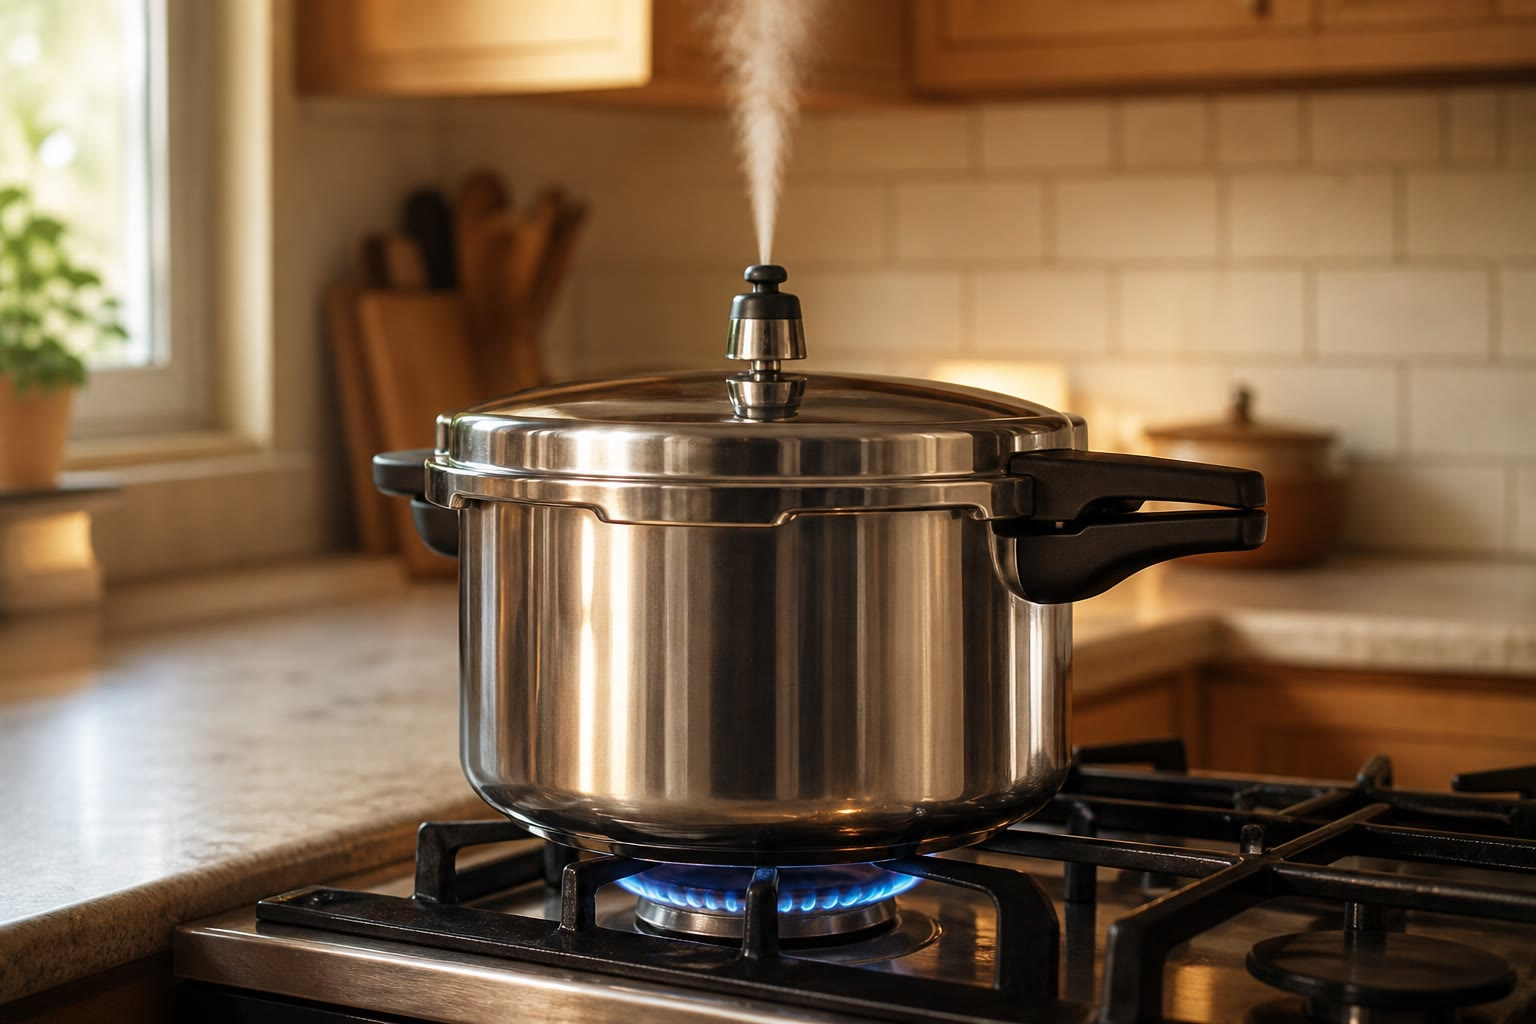
\includegraphics[width=0.58\linewidth]{images/book5/ai/b5-17-pressure-cooker.jpg}

{\small Un autocuiseur qui chuinte~: deux atmosphères à l'intérieur déplacent la ligne de coexistence liquide--vapeur à \qty{121}{\celsius} --- Clausius et Clapeyron, préparant le dîner plus vite.}
\end{omfigure}

\section{Problème~: le diagramme de phases de la cuisine}

\begin{problem}[{Problème du week-end --- autocuiseurs, thé de
montagne et la fin de l'ébullition}]\label{pb:b3:phase-transitions:1}
Le diagramme de phases de l'eau plane, inaperçu, au-dessus de chaque
cuisinière. Ce problème en parcourt les trois lignes, Clausius et
Clapeyron en main --- de la raison pour laquelle un autocuiseur
divise par deux les temps de cuisson, en passant par la déception du
thé en altitude, jusqu'au monde étrange au-delà du \omterm{prop:b3:phase-transitions:vdw}{point critique} où
l'ébullition elle-même cesse d'exister. Données~: $L_{\text{vap}}
= \qty{2.26e6}{J/kg}$, $L_{\text{fus}} = \qty{3.34e5}{J/kg}$~;
vapeur d'eau à \qty{373}{K}, \qty{1}{atm}~: $\Delta v_{\text{vap}}
= \qty{1.67}{m^3/kg}$~; fusion~: $\Delta v = \qty{-9.1e-5}{m^3/kg}$~;
masse moléculaire $m_{\text{w}} = \qty{3.0e-26}{kg}$~; \omterm{prop:b3:phase-transitions:vdw}{point
critique}~: $T_{\text{c}} = \qty{647}{K}$,
$P_{\text{c}} = \qty{221}{bar}$.

\medskip\noindent\textbf{Partie I --- La ligne d'ébullition.}
\begin{enumerate}
  \item Qu'est-ce qui définit l'«~ébullition~» à une pression
        donnée (quels deux \omterm{thm:b3:grand-canonical:distribution}{potentiels chimiques} s'égalisent)~?
  \item Calculer la pente $\dd P/\dd T$ de la ligne de
        vaporisation à \qty{100}{\celsius}.
  \item Un autocuiseur tient \qty{2}{atm}~: intégrer la pente (ou
        utiliser la forme exponentielle avec $Lm_{\text{w}}/
        k_{\text{B}} \approx \qty{4900}{K}$) pour trouver sa
        température d'ébullition.
  \item Avec la règle de cuisine d'Arrhenius de
        \cref{exo:b3:canonical-ensemble:9} (les vitesses doublent
        tous les \qty{10}{K}), estimer le gain de temps par rapport
        à la cuisson à casserole ouverte.
  \item À La Paz (\qty{3600}{m}, $P \approx \qty{0.65}{atm}$)~: la
        température d'ébullition, et pourquoi le thé y infuse mal.
  \item Pourquoi ajouter du sel élève-t-il le point d'ébullition
        (le $\mu$ de qui le soluté abaisse-t-il --- rappeler
        \cref{exo:b3:grand-canonical:8})~?
\end{enumerate}

\medskip\noindent\textbf{Partie II --- La ligne de fusion.}
\begin{enumerate}[resume]
  \item Calculer $\dd T/\dd P$ pour la fusion et noter le signe.
  \item Quelle observation quotidienne encode $\Delta v < 0$ (que
        fait la glace dans votre verre), et pourquoi cette anomalie
        est-elle rare parmi les substances~?
  \item Un glacier de \qty{300}{m} d'épaisseur~: la pression à sa
        base et l'abaissement du point de fusion --- la fusion sous
        pression basale compte-t-elle pour l'écoulement des
        glaciers~?
  \item Revenir au patineur de
        \cref{exo:b3:phase-transitions:7}(d)~: qu'est-ce qui
        lubrifie réellement la lame~?
  \item Si la glace coulait (pente positive, comme presque tout
        autre solide), que ferait l'hiver aux lacs et à leurs
        poissons --- dérouler la chaîne de conséquences.
  \item La pente négative s'arrête à haute pression, où d'autres
        formes cristallines de la glace prennent le relais (glaces
        III, V, VI)~: que dit l'existence d'une douzaine de glaces
        sur le paysage d'\omterm{prop:b3:canonical-ensemble:machine}{énergie libre} d'une seule molécule
        simple~?
\end{enumerate}

\medskip\noindent\textbf{Partie III --- Le bout de la ligne.}
\begin{enumerate}[resume]
  \item La ligne d'ébullition se termine en ($T_{\text{c}},
        P_{\text{c}}$)~: qu'advient-il de la chaleur latente et de
        la différence de densité à l'approche de ce bout~?
  \item Au-delà du \omterm{prop:b3:phase-transitions:vdw}{point critique}, on peut mener l'eau du régime
        «~liquide~» au régime «~gazeux~» sans \emph{aucune}
        transition~: décrire le chemin dans le plan $(P, T)$.
  \item À l'approche du \omterm{prop:b3:phase-transitions:vdw}{point critique}, le fluide devient
        laiteux~: relier cette opalescence à
        \cref{exo:b3:microcanonical-ensemble:12} et à
        \cref{pb:b3:perturbation-theory:1}.
  \item Le CO$_2$ supercritique ($T_{\text{c}} = \qty{304}{K}$,
        $P_{\text{c}} = \qty{74}{bar}$) dissout comme un liquide et
        pénètre comme un gaz~: nommer l'usage industriel qui
        décaféine le café, et dites pourquoi ce solvant ne laisse
        aucun résidu.
  \item L'eau supercritique (dans les chaudières des centrales
        au-dessus de \qty{221}{bar})~: pourquoi supprimer
        l'ébullition --- bulles, films, caléfaction --- séduit-il
        les ingénieurs des chaudières~?
  \item Les sources hydrothermales des grands fonds émettent de
        l'eau à \qty{400}{\celsius} qui ne bout pas~: vérifier face
        à la pression locale ($\sim\qty{300}{bar}$ à \qty{3}{km})
        et au diagramme de phases.
\end{enumerate}

\medskip\noindent\textbf{Partie IV --- Lire toute la carte.}
\begin{enumerate}[resume]
  \item Esquisser (en mots) le diagramme $(P, T)$ de l'eau~: les
        trois lignes, le point triple ($\qty{0.01}{\celsius}$,
        \qty{611}{Pa}), le \omterm{prop:b3:phase-transitions:vdw}{point critique}.
  \item Sous \qty{611}{Pa}, la glace se sublime sans fondre~: quel
        appareil (la lyophilisation) et quelles calottes polaires
        planétaires (Mars, CO$_2$ et H$_2$O) vivent de ce fait~?
  \item Pourquoi le point triple de l'eau --- exactement
        \qty{273.16}{K} par définition jusqu'en 2019 --- était-il
        un si bon étalon de température (combien de phases
        coexistantes fixent combien de \omterm{def:b3:lagrangian-mechanics:coordinates}{degrés de liberté})~?
  \item Chaque ligne de la carte est une transition du premier
        ordre~; seul son point terminal est critique~: reformuler la
        distinction avec les \omterm{def:b3:phase-transitions:order}{paramètres d'ordre} et la chaleur
        latente.
  \item La ligne de rosée de l'air humide, c'est la même physique
        jouée à l'envers~: expliquer la rosée, le brouillard et la
        buée du matin sur une vitre froide en une phrase de
        franchissement de $\mu$.
  \item Chaque couvercle de casserole est une expérience~: des
        gouttelettes s'y condensent et retombent en pluie ---
        identifier les deux \omterm{def:b3:phase-transitions:order}{transitions de phase} de ce cycle de
        l'eau miniature et la navette de chaleur latente qui fait
        bouillir plus tôt une casserole couverte.
  \item Résumer le résultat nommé~: une seule formule de pente,
        $\dd P/
        \dd T = L/T\Delta v$, explique les \qty{121}{\celsius} de
        l'autocuiseur, le thé à \qty{88}{\celsius} de la montagne,
        la glace qui remonte à l'envers sa ligne de fusion, et la
        bouilloire supercritique où l'ébullition s'arrête à
        $\qty{647}{K}, \qty{221}{bar}$.
\end{enumerate}
\end{problem}
